\documentclass[10pt,twocolumn]{article}

% use the oxycomps style file
\usepackage{oxycomps}

% usage: \fixme[comments describing issue]{text to be fixed}
% define \fixme as not doing anything special
\newcommand{\fixme}[2][]{#2}
% overwrite it so it shows up as red
\renewcommand{\fixme}[2][]{\textcolor{red}{#2}}
% overwrite it again so related text shows as footnotes
%\renewcommand{\fixme}[2][]{\textcolor{red}{#2\footnote{#1}}}

% read references.bib for the bibtex data
\bibliography{references}

% include metadata in the generated pdf file
\pdfinfo{
    /Title (GitHub Command Line Tutorial)
    /Author (Jesus Cornejo)
}

% set the title and author information
\title{GitHub Command Line Tutorial}
\author{Jesus Cornejo}
\affiliation{Occidental College}
\email{cornejoj@oxy.edu}

\begin{document}

\maketitle
\section{Prerequisites}
To follow along with this tutorial it is recommended that you have:
- A basic understanding of the command line
- Git installed and GitHub account set up
\section{What is Git?}
Git is a powerful tool used in software development that allows you to keep track of the changes you make to your files, and lets you share them with other developers who work on the same project. Git is a distributed system, meaning that each developer has a copy of the entire code history on their own computer. 
\section{Getting Started:}
To start we will create a new repository on GitHub.
A repository is where you store and manage your files using Git. A repository tracks the history and changes of your files, and allows you to work with other developers on the same project.
It should look like this: 

\begin{figure}[h!]
\center
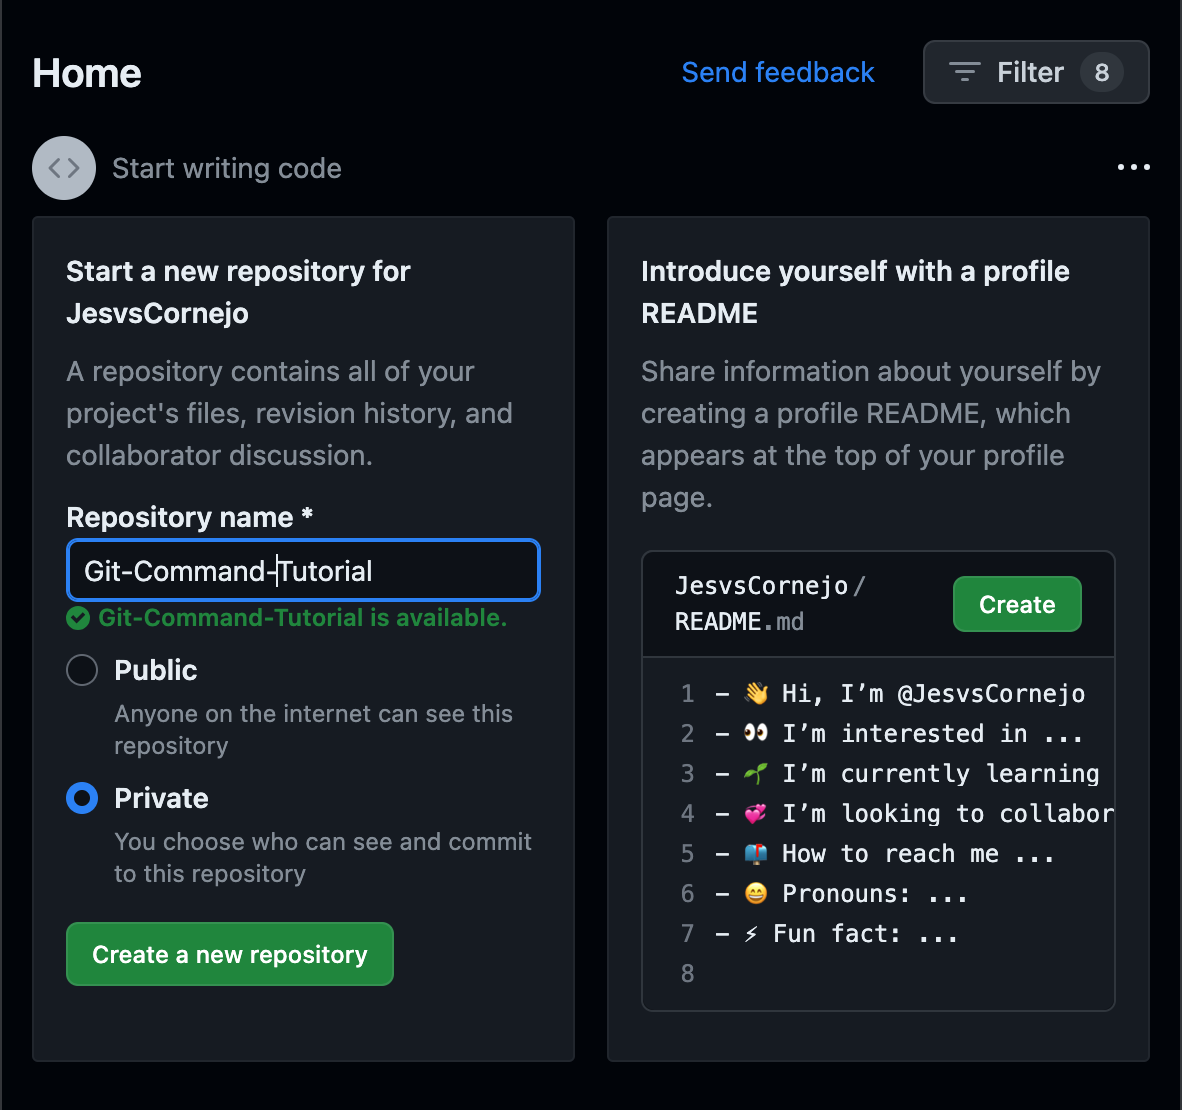
\includegraphics[width=0.5\textwidth]{screenshots/sc1.png}
\end{figure}

Once you've created a repository we can clone it to your computer using the command line with the command:  \textbf{git clone [URL]}\\
You can find and copy the link to the URL of your repository on GitHub by left-clicking on the tab \textbf{Code}.\\

\section{Creating a File:}
In order to access and work within your repository use the 'cd' command:  \textbf{cd *repository name*}\\
At this point there are no files in the repository. Let's start by making a python file using the 'mkdir' command\\
\textbf{mkdir *your file name*} I named my file heyGit.py\\
Once you successfully make the file you can use the 'ls -la' command to see the file in the repository.\\
It should look something like this:

\begin{figure}[h!]
\center
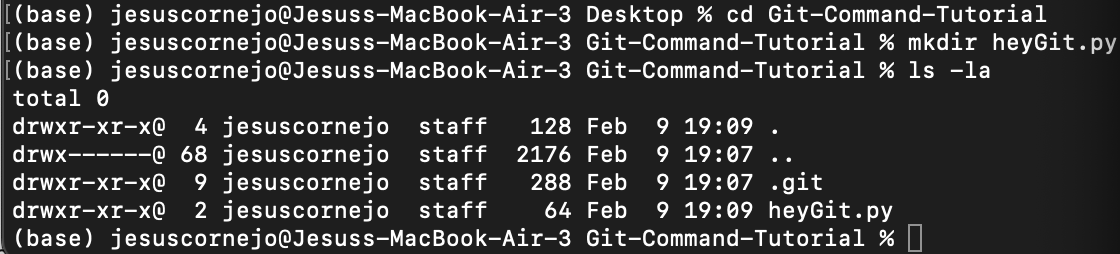
\includegraphics[width=0.5\textwidth]{screenshots/sc2.png}
\end{figure}

\section{Editing Files:}
Now that we have a python file in our repository, we can learn how to edit the file and then we'll be able to commit our first changes in the repository.\\
To edit the file we use the 'vim' command: \textbf{vim *file name*} A new window will open, you must hit the ‘i’ key first to insert and write code. Then hit the 'escape' key and type '\textbf{:wq}' (write and quit) at the bottom to save your changes.\\ \\
For my heyGit.py file I added a simple print statement.

\begin{figure}[h!]
\center
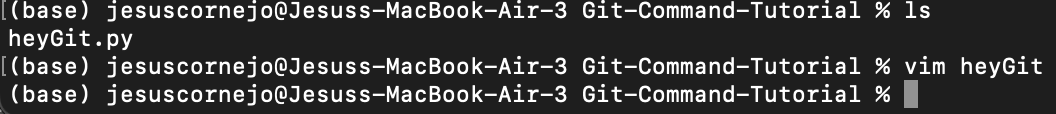
\includegraphics[width=0.5\textwidth]{screenshots/sc3.png}
\end{figure}

\begin{figure}[h!]
\center
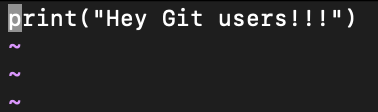
\includegraphics[width=0.5\textwidth]{screenshots/sc4.png}
\end{figure}

\newpage

\section{Committing:}
Now let's use the '\textbf{git status}' command to show us the changes we made to the file

\begin{figure}[h!]
\center
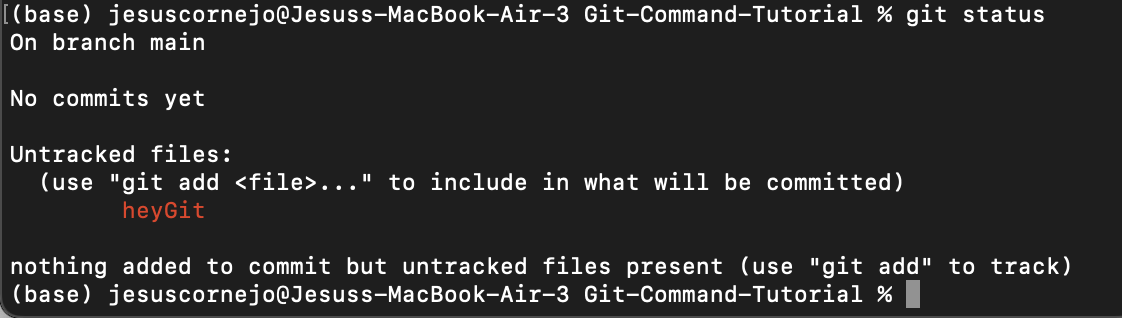
\includegraphics[width=0.5\textwidth]{screenshots/sc5.png}
\end{figure}

Here we see that I made a change, my untracked file: \textbf{heyGit}\\
Our next step is to commit the changes, but first we need to move our files to the staging area. The staging area, also known as index, is where you can selectively choose which changes to include in the next commit. By using the command:'\textbf{git add -A}' we add all files to the staging area.\\
Once we've added the file to the staging area we can commit to the repository using: '\textbf{git commit -m “Commit message”}'\\
The commit message should describe the changes you are committing in some way. For example I used the message: 'git commit -m "initial commit". Once you’ve successfully committed it should look like this:

\begin{figure}[h!]
\center
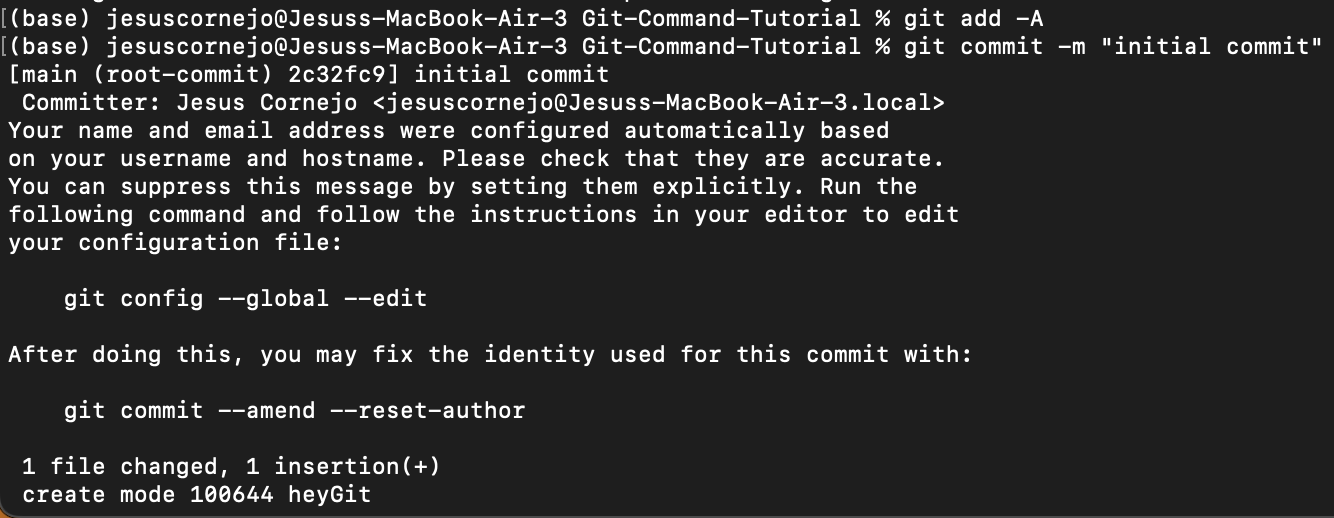
\includegraphics[width=0.5\textwidth]{screenshots/sc6.png}
\end{figure}

\newpage

\section{Branches:}
Now that we have a repository and have committed a file, lets take a look at branches in Git. Branches allow you to develop features, fix bugs, and safely experiment with new ideas in a contained area of your repository. The master or "\textbf{main}" branch remains stable while you or other developers work on different branches simultaneously.\\
To show the use of branching lets start by cloning this repository into a remote one. First we make a new repository just like before. I created the repository: \textbf{Git-Command-Remote} and have it cloned locally to my computer. Before we clone the old repository, we need to start by moving into our new remote repository using the 'cd' command: \textbf{cd Git-Command-Remote}.\\ \\
If we clone our old repository into this remote one now we may run into an error since there is a .git file already in our repository (you can use the \textbf{ls -a} command to see the file).\\
We can get around this error using the command: \textbf{rm -rf .git}. This will remove the first .git files that are causing the error. \\
After deletion we can now clone the old repository, but in this case we use the git clone command like this: 'git clone \textbf{../Git-Command-Tutorial .}' instead of using the URL link. 

\begin{figure}[h!]
\center
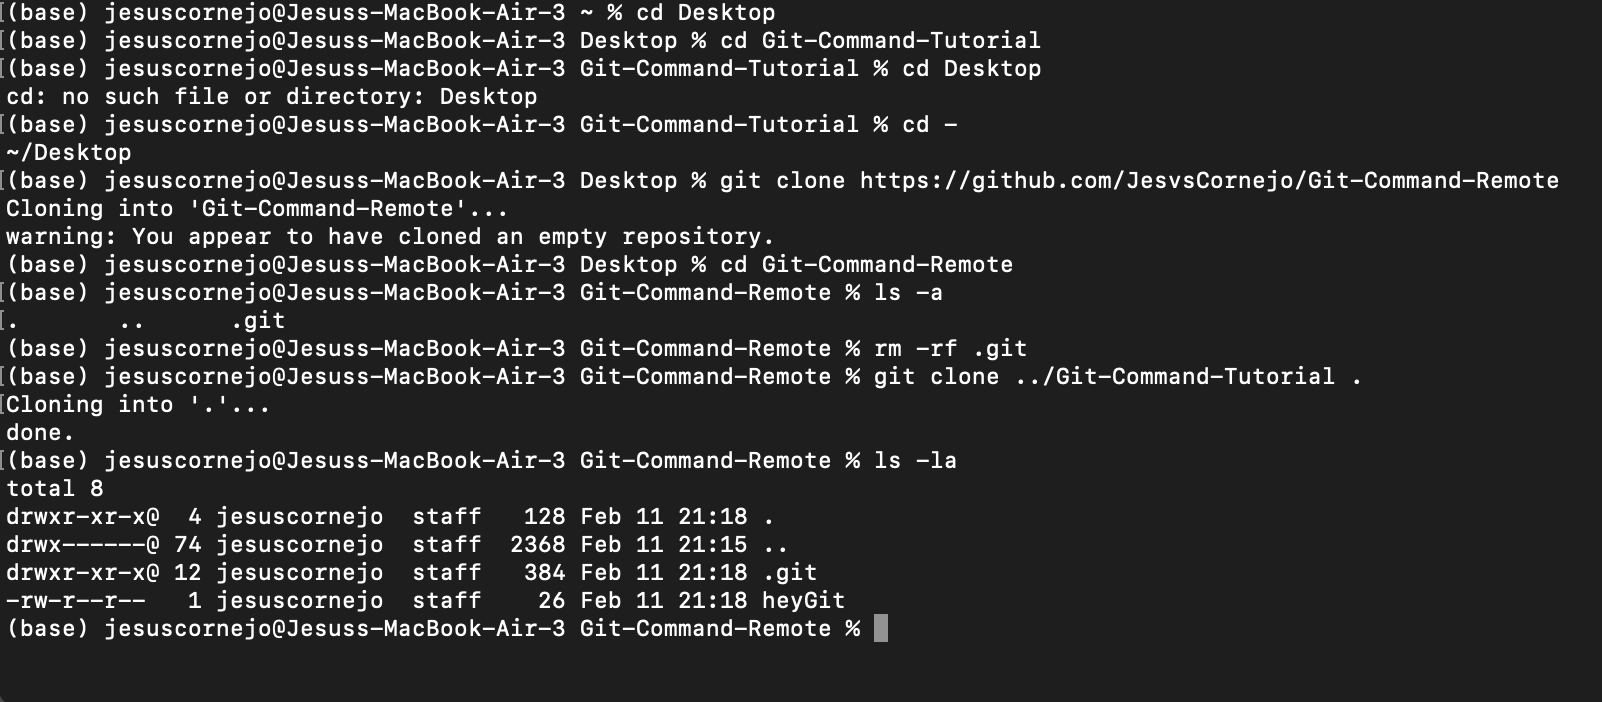
\includegraphics[width=0.5\textwidth]{screenshots/sc7.png}
\end{figure} 

We see that our remote repository now has the heyGit.py file. Lets edit this file and see how we can push changes using branches. Using the \textbf{vim} command again I simply added another print statement:
\begin{figure}[h!]
\center
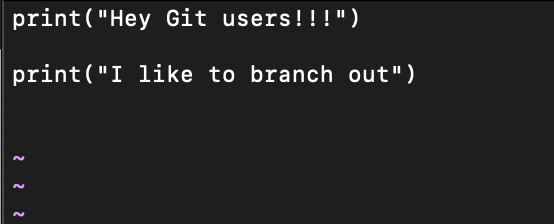
\includegraphics[width=0.5\textwidth]{screenshots/sc8.png}
\end{figure}


\newpage Now before we push our changes to our target repository we need to create a temporary branch in the old repository. To do this, we must navigate our way to the old repository using the 'cd' commands\\
Then use the command: \textbf{git checkout -b [temporary branch name]}. Now that we're on a new branch we can head back to the remote repository and use the command: \textbf{git push}\\

\begin{figure}[h!]
\center
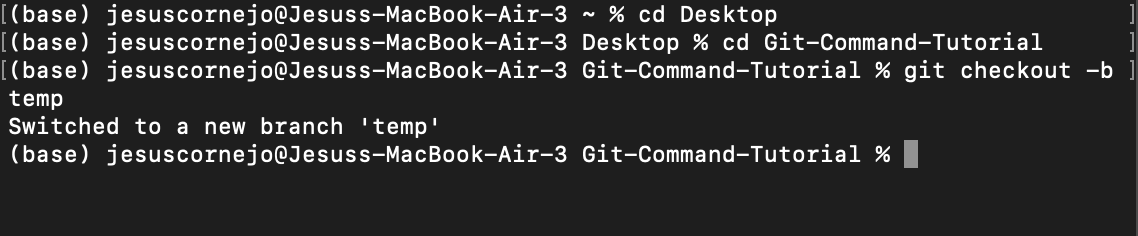
\includegraphics[width=0.5\textwidth]{screenshots/sc9.png}
\end{figure}

Up until now we have been working on our main branch, but now we'll create a new branch for us to work in. Use the command: \textbf{git branch *name of new branch*} to create a new branch in the repository.\\
We can use the \textbf{git branch} command without the name to see all of the branches in the repository. Here you can see my new branch which I named \textbf{heyGitBranch} then I used the command: \textbf{git checkout -name of branch-} to move into the new branch. My new branch is highlighted:\\

\begin{figure}[h!]
\center
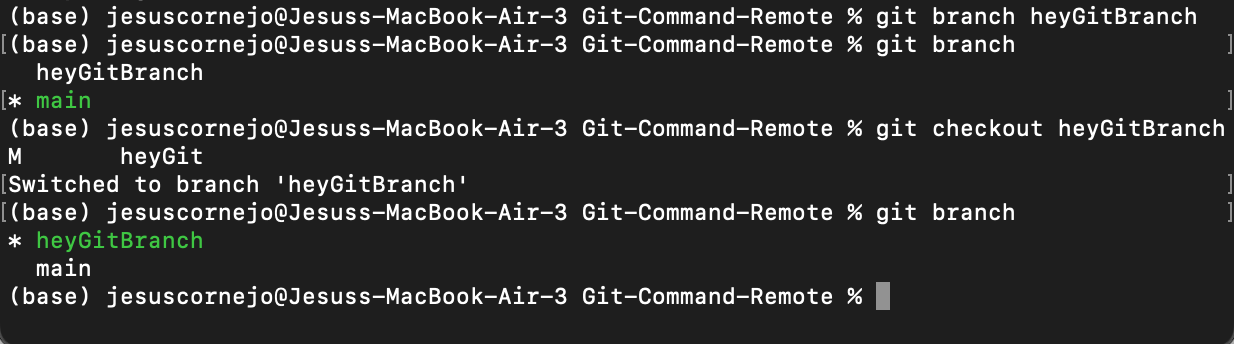
\includegraphics[width=0.5\textwidth]{screenshots/sc10.png}
\end{figure}


\newpage

\section{Merging:}
Once you've finished doing work on a branch it is sometimes beneficial for developers to merge branches back to the main branch. We will start by making some changes to our python file on our new branch. Once again, I added a simple print statement and now we will commit just like we did before.

\begin{figure}[h!]
\center
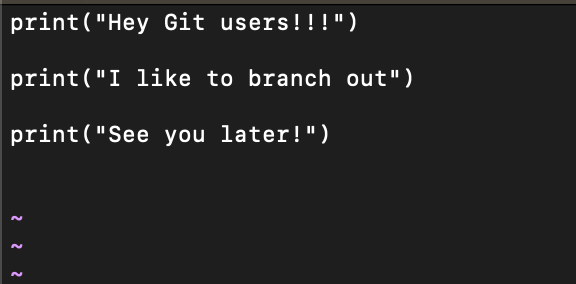
\includegraphics[width=0.5\textwidth]{screenshots/sc11.png}
\end{figure}

After committing let's push this branch to our original repository, to do that use the command: \textbf{git push -u origin *branch name*}

\begin{figure}[h!]
\center
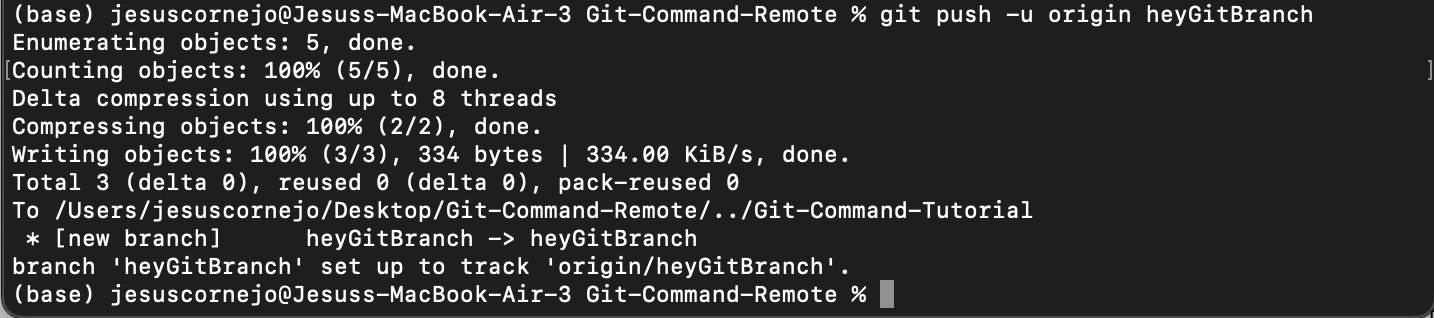
\includegraphics[width=0.5\textwidth]{screenshots/sc12.png}
\end{figure}

Now that we've made the changes on one branch, lets see how we can merge our two branches.\\
First move back into our main branch using our checkout command: \textbf{git checkout main}. If we use the command: \textbf{git branch --merged} we will only see our main branch since we haven’t merged our new one\\

\begin{figure}[h!]
\center
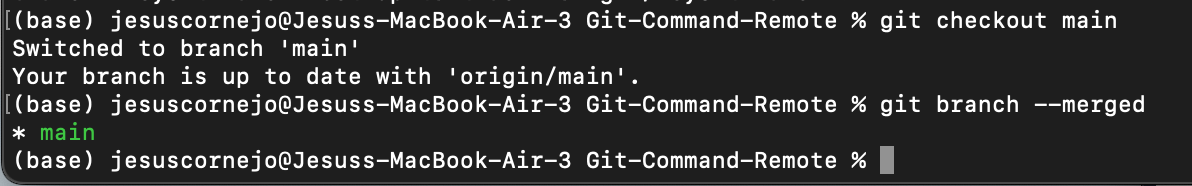
\includegraphics[width=0.5\textwidth]{screenshots/sc13.png}
\end{figure}

So let's merge our branches! Use the command: \textbf{git merge *name of branch*}\\ \\
Then push to the original repository using the command: \textbf{git push origin main}

\begin{figure}[h!]
\center
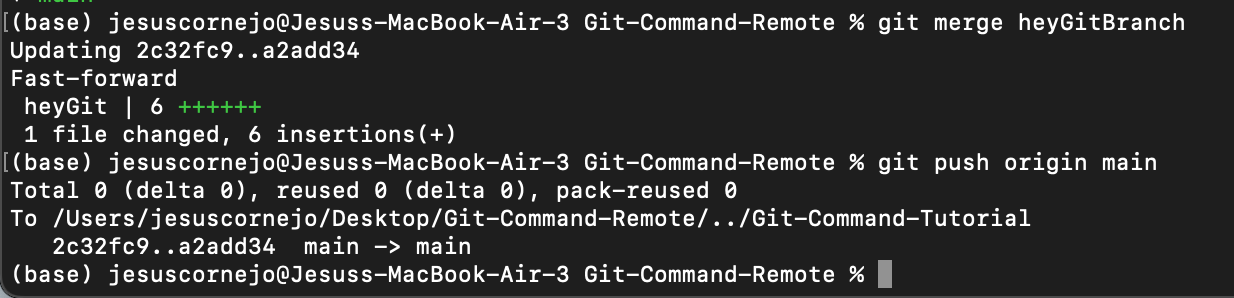
\includegraphics[width=0.5\textwidth]{screenshots/sc14.png}
\end{figure}

\subsection{Deleting Branches:}
Now that we've merged into main we can delete our branch. Use the command: \textbf{git branch -d [name of branch]}\\
Once the branch is deleted locally we need to delete it from the original repository. Use the command: \textbf{git push origin --delete [name of branch]} \\

\begin{figure}[h!]
\center
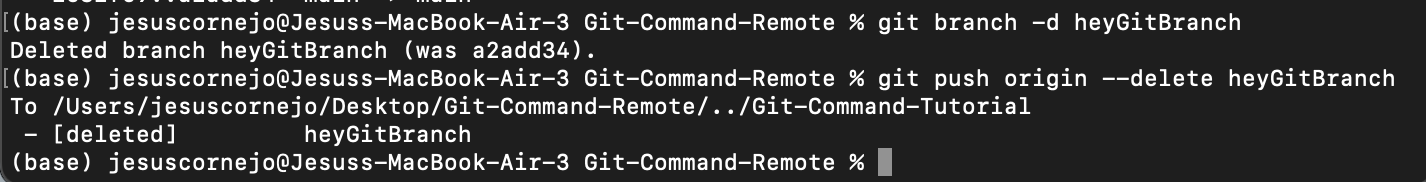
\includegraphics[width=0.5\textwidth]{screenshots/sc15.png}
\end{figure}

\newpage

\section{Stashes:}
After looking at how branches and commits work, we should also learn how to save our work when its not ready to commit.\\
Stashes are really useful in this case because they temporarily shelve changes you've made to your working copy so you can work on something else, and then come back and re-apply them later on. To show this, let's make a change on our python file using 'vim' command. Once the file has changes made we can use the \textbf{git status} command to see the change:

\begin{figure}[h!]
\center
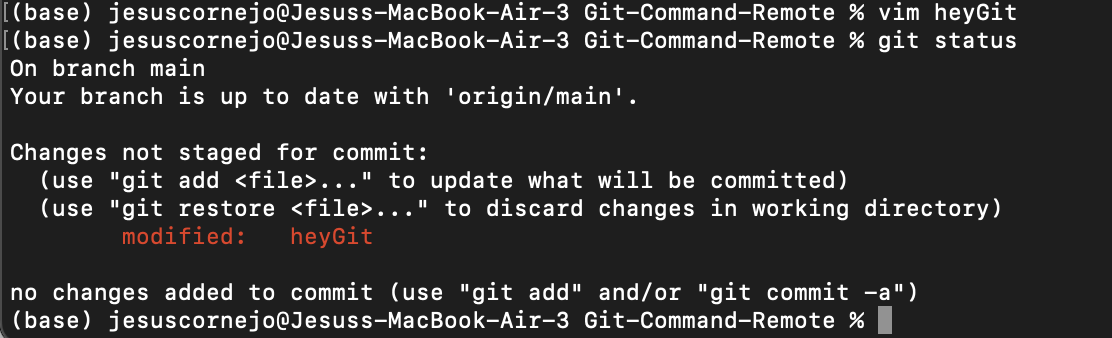
\includegraphics[width=0.5\textwidth]{screenshots/sc16.png}
\end{figure}

Here we see that the file has changed but is not staged or committed. Let's say that now we want to change branches and work on something else. We can use the command '\textbf{git stash}' to save our work so we can reapply it later.\\

\begin{figure}[h!]
\center
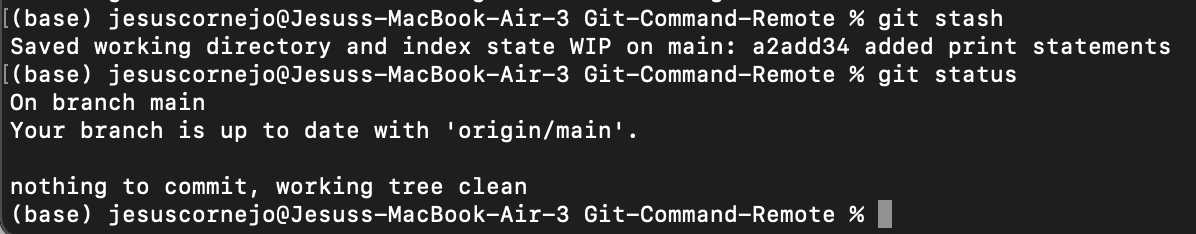
\includegraphics[width=0.5\textwidth]{screenshots/sc17.png}
\end{figure}

Here we see that, after stashing, our working tree is clean and our changes are saved.

\newpage

\subsection{Saved Stashes:}
To bring back our work we can use the command: \textbf{git stash apply}\\

\begin{figure}[h!]
\center
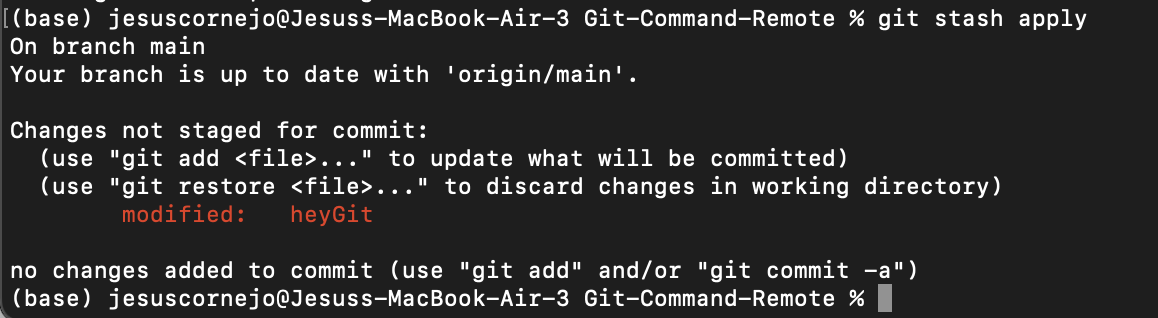
\includegraphics[width=0.5\textwidth]{screenshots/sc18.png}
\end{figure}

Here we see that we are back to our original state with our changes ready to be staged and committed.




\end{document}
